\documentclass{article} % For LaTeX2e
\usepackage{nips15submit_e,times}
\usepackage{hyperref}
\usepackage{url}
\usepackage{amsmath}
\usepackage{graphicx}
%\documentstyle[nips14submit_09,times,art10]{article} % For LaTeX 2.09


\title{Implementation and Analysis of Random Forests}


\author{
Jae Lee\\
School of Computing Science\\
Simon Fraser University\\
Burnaby BC V5A 1S6 \\
%\texttt{email} \\
\And
Richard Mar \\
School of Computing Science\\
Simon Fraser University\\
Burnaby BC V5A 1S6 \\
%\texttt{email} \\
\AND
Robin White \\
School of Mechatronic Systems Engineering\\
Simon Fraser University\\
Surrey BC V3T 0A3 \\
%\texttt{email} \\
}

\newcommand{\fix}{\marginpar{FIX}}
\newcommand{\new}{\marginpar{NEW}}

\nipsfinalcopy % Uncomment for camera-ready version

\begin{document}


\maketitle

\begin{abstract}
TODO: Decide if we need this section.
\end{abstract}

\section{Introduction}


In machine learning, there is often a tug-of-war between bias and variance; having high accuracy to observed data but not to lose generalization (or over-fit) to unseen data. This is often referred to as the "bias-variance tradeoff" and it's consideration is a significant part of properly engineering machine learning algorithms. Often, regularization is used where there is an addition to the loss function to represent a cost to complexity, or in the way of neural networks, random dropout of neurons to force generalization \cite{Srivastava2014}. Another method is to also use validation datasets so as to understand the loss from unseen data without actually testing on the test set. All of these methods add to the complexity of the algorithm and can also often lead to loss in accuracy of the training data.\\
In the early 90's, Tin Kam Ho from Bell Labs published a series of papers where he showed surprisingly that by combining independent learners in a unique way increased the accuracy of classifying handwritten digits monotonically; without suffering from over-adaptation to the training data. \cite{Ho93, Ho95, Ho98} The application of this method to decision trees in his '93 paper marked the introduction of Random Forests to the community. \cite{Ho93} Decision trees are simple yet effective classifiers, with high execution speed and easily relatable, however they are limited by their complexity for possible loss of generalization to unseen data. Some methods such as pruning have been used previously to try and increase generalization, however methods such as these usually come with a loss in accuracy toward training data. By using principles of stochastic modeling, Ho showed that tree-based classifiers could be arbitrarily expanded for increases in accuracy on unseen testing data without loss in training data accuracy. A characteristic which is still unique among machine learning classifiers. The concept is that multiple learners can compensate for the bias of a single learner and so trees are constructed from randomly selecting subspaces of the feature space. In this way, each tree generalizes in a different way. \\
Random Forests have been applied to a variety of machine learning tasks including classifications in ecology and geosciences, image segmentation in medical applications, business analytics, sporting analytics, as well as the unmentioned number of general data science applications. \cite{Cutler2007, Harris2015, Luo2017, Ghatasheh2014, Lock2014} In this report we aim to investigate the application of Random forests as classifier and regressor to a hockey player dataset. We present the general algorithm coded in python, as well as investigate the various parameters such as number of trees, number of features per tree, and splitting criteria comparing entropy and Gini impurity for classification, and variance for regression. We also compare results of our algorithm to that of sci-kit learn and Weka, and discuss key similarities and differences. We conclude with discussion on limitations and challenges in present work on Random forests.

\subsection{Decision Trees}
TODO: Outline general Decision tree algorithm.

\subsection{Random Forests}
TODO: Outline general Random forest algorithm. Pseudo code

\subsection{Ensemble Learning}
TODO: Decide what content to go where

Randomization increases bias but makes it possible to reduce the variance of the corresponding ensemble model through averaging. \cite{formann-roe_2012}

\textbf{Bootstrap Aggregating (Bagging)}

Bootstrap aggregating or bagging is an ensemble learning technique that attempts to reduce variance of the model without increasing the bias by attempting to remove correlation between individual trees. Each tree is limited to evaluating only a random fractional sample of the actual dataset such that no two samples are the same. Bagging has been demonstrated empirically to improve model accuracy. \cite{Aslam07}\\

From the actual dataset D of size n, k bootstrap samples, \[ D_1,D_2,..D_k  \] are randomly selected with repetition from D.

Then the variance of the ensemble is the average of the sum of the individual trees' variances.

\[ var(L) = \frac{\sum_{i=1}^k var(L_i)}{k}\] where L is the ensemble of individual learners (trees).\\

Each datapoint in D has a probability of \[1-\left(\frac{1}{n}\right)^n = e^{-1} \approx 36.8 \% \] of not being selected in  a sample D\textsubscript{i} and therefore approximately 63.2\% probability of being in a training set D\textsubscript{i}.

\section{Approach}
TODO: Figure out what is supposed to be here.

\section{Experiments}
TODO: Add content.

\subsection{Forest Size}
TODO: Add content.

\subsection{Tree Depth}
TODO: Add content.

\subsection{Splitting Criteria}

\textbf{Random Subspace Method}

Random forest uses a modified splitting algorithm that attempts to further reduce correlation between individual trees. For example, if few attributes are strong predictors of the target label, these attributes will be selected in many trees leading to high correlation and greater generalization error.  Generalization error of an ensemble converges to the following expression:

\[Generalization\ error \leq \frac{corr(1-s^2)}{s^2}\] where corr is the average correlation among the trees and s is the average performance of individual classifiers. Thus, reducing correlation among the individual trees will also lower the generalization error.

 Work by Ho has demonstrated that average tree agreement between trees is significantly lowered using the Random subspace method. \cite{Ho98}
Estimating tree agreement between trees i and j as s\textsubscript{i,j}

\[ s_{i,j} = \frac{1}{n}\sum_{k=1}^{n}f(x_k)\]
\
\[ where \ f(x_k) = \begin{cases}
      1 & if\ class\ decision_i(x_k) = class \ decision_j(x_k) \\
      0 & otherwise
   \end{cases}
\]

Ho's result showed average of s\textsubscript{i,j} of random subspaces method was lower than that of bootstrapping and boosting methods alone. \cite{Ho98}

 Thus, limiting a tree's evaluation to only a fixed size subset of the actual features and randomizing the elements in the subset during each splitting process helps to reduce correlation among each trees. The modified splitting algorithm will then split on a single feature with the best information gain ratio or gini impurity to reduce correlation among trees.

\subsubsection{Entropy}
TODO: Add content.

\subsubsection{Gini Index}
Gini impurity index measures the probability of incorrectly labeling an element if it was randomly labeled according to the distribution of labels in the leaf node. Gini impurity and Entropy are analogous. Gini impurity is less computationally expensive since it doesn't require calculating logarithmic functions.

Given k classes and fraction of elements in the leaf node with class i, p\textsubscript{i}, the Gini impurity can be calculated as:
\[G(p) = \sum_{i=1}^{k}p_i \sum_{j=1}^{k}p_j = \sum_{i=1}^{k}(p_i-p_i^2) = 1 - \sum_{i=1}^{k}p_i^2 \]

\subsection{Custom Improvement?}



\begin{figure}[h]
\begin{center}
%\AddToShipoutPicture see eso-pic
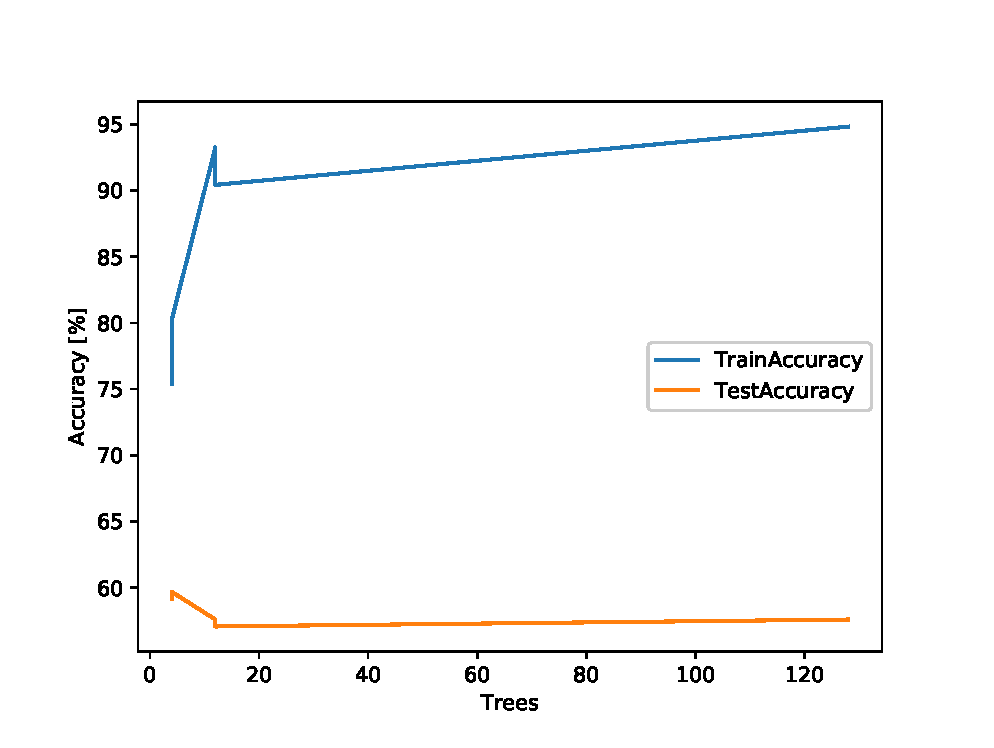
\includegraphics{TrainTestClassifierAcc}
%\framebox[4.0in]{$\;$}
%\fbox{\rule[-.5cm]{0cm}{4cm} \rule[-.5cm]{4cm}{0cm}}
\end{center}
\caption{Showing Random forest inhibition to produce overfitting errors even with incresed complexity by large number of trees.}
\end{figure}

%Can't get it to center this table...
\begin{table}[t]
\caption{Optimal values found for sci-kit learn Random forest by grid search}
\begin{center}
\begin{tabular}{cccccc}
{\bf Target class} &{\bf Max depth} &{\bf Num features} &{\bf Min samples per leaf} &{\bf Min samples for split} &{\bf Num of trees}
\\ \hline \\
GP\_greater\_than\_0         &8	&5	&2	&2	&128 \\
sum\_7yr\_GP         &8	&5	&4	&2	&64 \\
\label{scikit-table}
\end{tabular}
\end{center}
\end{table}


\begin{table}[t]
\caption{Comparison of Random forest classifier for GP\_greater\_than\_0}
\label{clas-table}
\begin{center}
\begin{tabular}{lll}
\multicolumn{1}{c}{\bf Machine Learning Package} &\multicolumn{1}{c}{\bf Accuracy} &\multicolumn{1}{c}{\bf Time}
\\ \hline \\
Weka         &56\%	&$<$1sec \\
scikit-learn             &55\%	&TIME \\
our implementation             &57\%	&$\approx$ 3min \\

\end{tabular}
\end{center}
\end{table}

From Table~\ref{clas-table}, it can be seen that all three implementations of Random forest yield similar results. It was noted however that when performing Weka on a unprocessed data set, that is without changing the country group to binary dummy features, as well as without standardization of the feature vectors, the Weka accuracy yielded 69\% accuracy, compared to the 56\% accuracy. (TODO: Comment on possibilities, multi-class splitting? WIll investigate at what point do we see loss in accuracy). The time taken for completion is difficult to compare since coding implementations are different, however using 4 workers running using the same parameters as shown in table ~\ref{scikit-table} the time of 3 minutes is slow, however not unreasonable. 

Random forests have been shown to achieve high classification performance through ensemble with a set of decision trees that are constructed using randomly selected feature subspaces. The performance of an ensemble learner is dependent on the accuracy of each component learner and the diversity of the components, especially when using a small set of trees which may be limited due to computational cost. The randomization can cause occurence of bad predicting trees as well as correated trees which can lead to poor ensemble decisions, which can be observed when performing multiple training runs using the same parameters which can lead to different accuracy results. Attempts have been made to improve the performance of this model by building a forest of only uncorrelated high performing trees. \cite{Bharathidason2014}

\section{Conclusion}
TODO: Add content.


\subsubsection*{Contributions}
All authors contributed equally.\\
See GitLab project here for specific commits:\\
\href{
    https://csil-git1.cs.surrey.sfu.ca/rkm3/mlclass-1777-randomforest
}{
    https://csil-git1.cs.surrey.sfu.ca/rkm3/mlclass-1777-randomforest
}


\small{
\bibliography{report}
\bibliographystyle{ieeetr}
}

\end{document}
